\documentclass[conference]{IEEEtran}
\IEEEoverridecommandlockouts
% The preceding line is only needed to identify funding in the first footnote. If that is unneeded, please comment it out.
\usepackage{cite}
\usepackage{amsmath,amssymb,amsfonts}
\usepackage{algorithmic}
\usepackage{graphicx}
\usepackage{textcomp}
\usepackage{xcolor}
\usepackage{listings}
\usepackage{url}
\usepackage{booktabs}
\usepackage{array}
\usepackage{multirow}

\def\BibTeX{{\rm B\kern-.05em{\sc i\kern-.025em b}\kern-.08em
    T\kern-.1667em\lower.7ex\hbox{E}\kern-.125emX}}

\begin{document}

\title{US Corn Yield Prediction Using Multi-Source Data Integration and Machine Learning}

\author{\IEEEauthorblockN{Ahsan Riaz}
\IEEEauthorblockA{\textit{School of Electrical Engineering and Computer Sciences} \\
\textit{National University of Science and Technology}\\
Islamabad, Pakistan \\
ahsanriaz8000@gmail.com}
}

\maketitle

\begin{abstract}
Accurate prediction of crop yields is crucial for agricultural planning, food security assessment, and market forecasting. This paper presents a comprehensive machine learning system for predicting county-level corn yields across the United States by integrating heterogeneous datasets from multiple sources. We combine historical agricultural statistics from USDA NASS, weather data from NASA POWER, and soil properties from USDA NRCS to create a rich feature set of 50 variables. Our system employs multiple modeling approaches including Ridge Regression, Random Forest, Gradient Boosting, and XGBoost, with comprehensive hyperparameter tuning. The best-performing model (XGBoost) achieves an R² score of 0.863 and a mean absolute error of 11.22 BU/ACRE on test data, representing approximately 6.4\% relative error. Feature importance analysis reveals that historical yield patterns account for 53\% of predictive power, while weather anomalies and stress indicators contribute significantly to model performance. We develop an interactive web-based proof-of-concept application using Streamlit that enables users to explore predictions, analyze scenarios, and understand model insights. Error analysis demonstrates that the model performs best in major corn-producing regions and during typical weather conditions, with increased errors during extreme events such as the 2012 drought. Our results demonstrate the effectiveness of integrating multiple data sources and ensemble learning techniques for agricultural yield prediction.
\end{abstract}

\begin{IEEEkeywords}
Machine Learning, Crop Yield Prediction, Agricultural Data, Ensemble Methods, Feature Engineering, Time Series Forecasting
\end{IEEEkeywords}

\section{Introduction}

Agricultural yield prediction has long been a critical challenge in food security and agricultural economics. Accurate forecasts enable farmers to make informed decisions about resource allocation, help policymakers assess food availability, and support commodity markets in price discovery. Corn, being one of the most widely cultivated crops in the United States with over 90 million acres planted annually, represents an important case study for yield prediction systems.

Traditional yield prediction methods have relied heavily on expert knowledge, historical averages, and statistical models with limited predictive power. The advent of machine learning techniques, combined with increased availability of agricultural and environmental data, has opened new possibilities for more accurate and nuanced yield forecasting. However, effective yield prediction requires integrating information from multiple domains: historical agricultural performance, weather patterns, soil characteristics, and management practices.

This project addresses the challenge of predicting county-level corn yields across the United States by developing a comprehensive machine learning pipeline that integrates data from multiple public sources. We combine historical yield statistics, detailed weather information, and soil properties to create a rich feature representation of growing conditions. Our approach employs multiple machine learning algorithms and extensive hyperparameter tuning to achieve state-of-the-art performance.

The contributions of this work include: (1) a comprehensive data integration framework combining USDA NASS agricultural statistics, NASA POWER weather data, and USDA NRCS soil data; (2) extensive feature engineering including temporal lags, climate anomalies, and stress indicators; (3) a thorough comparison of multiple modeling approaches with rigorous evaluation; (4) detailed error analysis identifying model strengths and limitations; and (5) an interactive web application demonstrating practical utility of the system.

\section{Problem Definition}

The problem we address is predicting county-level corn yield (in bushels per acre) for a given year based on available data up to that point. This is a regression problem where the target variable is continuous and the input features include historical yields, weather conditions, soil properties, and geographic information.

Formally, given a county $c$, state $s$, and year $y$, we aim to predict:
\begin{equation}
\hat{Y}_{c,s,y} = f(X_{c,s,y}, H_{c,s,<y}, W_{c,s,y}, S_c)
\end{equation}
where:
\begin{itemize}
    \item $X_{c,s,y}$ represents weather features for county $c$ in year $y$
    \item $H_{c,s,<y}$ represents historical yield data for county $c$ prior to year $y$
    \item $W_{c,s,y}$ represents weather data for county $c$ in year $y$
    \item $S_c$ represents soil properties for county $c$ (assumed static)
\end{itemize}

The prediction must be made before harvest time, making this a forecasting problem that relies on in-season weather data and historical patterns.

\section{Related Work}

Crop yield prediction has been studied extensively using various approaches. Early work relied on statistical methods such as regression analysis and time series models \cite{schlenker2009nonlinear}. With the availability of remote sensing data, many studies incorporated satellite-derived vegetation indices such as NDVI \cite{becker2019using}. More recently, machine learning approaches including support vector machines \cite{crane2011forecasting}, random forests \cite{jeong2016random}, and neural networks \cite{pantazi2016wheat} have shown improved performance.

Several studies have integrated multiple data sources for yield prediction. Schwalbert et al. \cite{schwalbert2020forecasting} combined weather data with soil properties for soybean yield prediction in Brazil. Jeong et al. \cite{jeong2016random} used historical yields, weather, and soil data with random forests to predict corn and soybean yields. However, many existing studies focus on regional or state-level predictions rather than county-level granularity.

Recent work has explored deep learning approaches. Wang et al. \cite{wang2018deep} used convolutional neural networks with satellite imagery, while You et al. \cite{you2017deep} applied long short-term memory networks to capture temporal dependencies. However, these methods often require extensive data preprocessing and computational resources.

Our work distinguishes itself by: (1) integrating data from three major public sources at county-level resolution; (2) extensive feature engineering focusing on anomalies and stress indicators; (3) comprehensive model comparison including ensemble methods; and (4) development of an interactive application for practical use.

\section{Data Acquisition and Preparation}

\subsection{Data Sources}

We integrate data from four primary sources to create a comprehensive dataset:

\textbf{USDA NASS QuickStats:} County-level agricultural statistics including corn yield (BU/ACRE), area planted (ACRES), area harvested (ACRES), and total production (BU) for the period 1981-2023. This dataset provides the target variable and key agricultural metrics. Data was downloaded via the QuickStats API for all US counties reporting corn production.

\textbf{NASA POWER Agroclimatology:} Daily weather data including minimum, maximum, and mean temperature, precipitation, and relative humidity. We aggregate this to weekly resolution and calculate growing season metrics. The data covers the period 1981-2023 with global coverage at 0.5° × 0.625° resolution. We extract data for county centroids to obtain location-specific weather information.

\textbf{USDA NRCS Soil Data Access:} Soil properties including available water capacity (AWC), clay content percentage, soil pH, and organic matter percentage. These properties are relatively static and represent long-term soil characteristics. Data is available at the county level through the Soil Data Access web service.

\textbf{US Census TIGER/Line:} County geographic centroids used for spatial queries to extract weather data for each county location.

\subsection{Data Integration and Cleaning}

The integration process involves several steps:

\begin{enumerate}
    \item \textbf{Spatial Matching:} County centroids are used to extract weather data from the nearest NASA POWER grid point for each county.
    \item \textbf{Temporal Alignment:} All data sources are aligned by county and year to create county-year observations.
    \item \textbf{Data Quality Checks:} We identify and handle missing values, outliers, and inconsistencies. Counties with incomplete data or reporting discontinuities are flagged.
    \item \textbf{Feature Calculation:} Derived features such as abandonment rate and harvest efficiency are calculated from the raw agricultural data.
\end{enumerate}

The final integrated dataset contains 82,436 county-year observations spanning 1981-2023 across 2,635 counties in the continental United States. Each observation includes 50 features covering historical yields, weather patterns, soil properties, and geographic information.

\subsection{Data Split}

We use a temporal split to maintain temporal ordering and prevent data leakage:
\begin{itemize}
    \item Training set: 1981-2015 (70\%)
    \item Validation set: 2016-2019 (15\%)
    \item Test set: 2020-2023 (15\%)
\end{itemize}

This split ensures that models are evaluated on truly future data, which is essential for assessing real-world forecasting capability.

\section{Feature Engineering}

\subsection{Historical Yield Features}

Historical yield patterns are strong predictors of future yields due to persistent factors such as soil quality, management practices, and local climate adaptation. We create three lag features:
\begin{itemize}
    \item \textbf{Yield\_Lag1:} Yield from the previous year
    \item \textbf{Yield\_Lag2:} Yield from two years prior
    \item \textbf{Yield\_3yr\_Avg:} Three-year moving average of yields (excluding current year)
\end{itemize}

Feature importance analysis reveals these historical features account for 53\% of total predictive power, highlighting the importance of temporal patterns.

\subsection{Weather Features}

Weather data is aggregated into multiple features capturing different aspects of growing conditions:

\textbf{Temperature Features:} Growing degree days (GDD) calculated with base temperature of 10°C and maximum of 30°C, aggregated by growth stage (vegetative, reproductive, grain fill). Mean, maximum, and minimum temperatures for the growing season and critical reproductive period. Standard deviation and range of temperatures to capture variability.

\textbf{Precipitation Features:} Total precipitation and stage-specific precipitation (vegetative, reproductive, grain fill). Mean weekly precipitation, maximum weekly precipitation, and standard deviation. Counts of dry weeks (precipitation < 10mm) and wet weeks (precipitation > 40mm).

\textbf{Climate Anomalies:} We calculate deviations from county-specific 30-year normals (1991-2020) for GDD, precipitation, and temperature. Anomalies capture unusual conditions that may significantly impact yields:
\begin{equation}
\text{Anomaly} = \text{Actual Value} - \text{County Normal}
\end{equation}

Anomaly features prove more predictive than absolute values, as they account for local adaptation to typical conditions.

\subsection{Stress Indicators}

We develop composite features that capture stress conditions:

\textbf{Heat Stress:} Count of weeks with maximum temperature exceeding 32°C (heat stress threshold) and 35°C (extreme heat).

\textbf{Water Stress:} Combined indicator of low precipitation and high temperature during the critical reproductive period:
\begin{equation}
\text{Water Stress} = \frac{32 - T_{\text{repro}}}{P_{\text{repro}}/10 + 1}
\end{equation}
where $T_{\text{repro}}$ is reproductive period temperature and $P_{\text{repro}}$ is reproductive period precipitation.

\textbf{Heat-Moisture Stress:} Combined indicator capturing interactions between heat and moisture:
\begin{equation}
\text{Heat-Moisture Stress} = \frac{\text{Weeks Heat Stress}}{\text{Total Precip}/100 + 1}
\end{equation}

\subsection{Soil Features}

Soil properties (AWC, clay content, pH, organic matter) are included as static features for each county. While less dynamic than weather features, they provide important baseline information about soil quality and water-holding capacity.

\subsection{Geographic Features}

State is encoded as a categorical feature to capture regional patterns in growing practices, varieties, and climate zones.

\section{Methodology}

\subsection{Baseline Model}

We establish a baseline using a simple 3-year moving average of historical yields for each county:
\begin{equation}
\hat{Y}_{c,y} = \frac{1}{3}\sum_{i=1}^{3} Y_{c,y-i}
\end{equation}

This baseline achieves an R² of 0.628 on test data, providing a benchmark for more sophisticated models.

\subsection{Classical Machine Learning Models}

\textbf{Ridge Regression:} A linear model with L2 regularization to prevent overfitting. Features are standardized using StandardScaler. Hyperparameters are tuned via grid search over regularization strength $\alpha \in \{0.1, 1.0, 10.0, 100.0, 1000.0\}$.

\subsection{Ensemble Methods}

\textbf{Random Forest:} An ensemble of decision trees with bootstrap sampling and feature subsetting. Hyperparameters tuned via randomized search:
\begin{itemize}
    \item Number of estimators: \{100, 200, 300, 400\}
    \item Maximum depth: \{10, 20, None\}
    \item Minimum samples split: \{2, 5, 10\}
    \item Minimum samples leaf: \{1, 2, 4\}
    \item Maximum features: \{'auto', 'sqrt', 'log2'\}
\end{itemize}

\textbf{Gradient Boosting:} Sequential ensemble method that builds trees to correct previous errors. Hyperparameters include learning rate (0.01-0.3), number of estimators (100-500), maximum depth (3-10), and subsample ratio (0.8-1.0).

\textbf{XGBoost:} Optimized gradient boosting implementation with additional regularization. Key hyperparameters include learning rate (0.01-0.3), maximum depth (3-10), minimum child weight (1-7), subsample (0.6-1.0), and column subsample (0.6-1.0).

\subsection{Hyperparameter Tuning}

Hyperparameter optimization is performed using 5-fold cross-validation on the training set. For Random Forest, Gradient Boosting, and XGBoost, we use RandomizedSearchCV with 12-20 iterations to balance exploration and computational efficiency. Ridge Regression uses GridSearchCV due to smaller parameter space. The best model from validation performance is selected for final evaluation on the test set.

\subsection{Feature Scaling}

Linear models (Ridge) require feature scaling, which is performed using StandardScaler fitted on training data and applied to validation and test sets. Tree-based methods (Random Forest, Gradient Boosting, XGBoost) do not require scaling and are trained on raw feature values.

\section{Experimental Setup}

\subsection{Evaluation Metrics}

Model performance is assessed using three metrics:

\textbf{R² Score (Coefficient of Determination):} Measures the proportion of variance explained:
\begin{equation}
R^2 = 1 - \frac{\sum_{i}(y_i - \hat{y}_i)^2}{\sum_{i}(y_i - \bar{y})^2}
\end{equation}

\textbf{Mean Absolute Error (MAE):} Average magnitude of prediction errors:
\begin{equation}
\text{MAE} = \frac{1}{n}\sum_{i=1}^{n}|y_i - \hat{y}_i|
\end{equation}

\textbf{Root Mean Squared Error (RMSE):} Penalizes larger errors more heavily:
\begin{equation}
\text{RMSE} = \sqrt{\frac{1}{n}\sum_{i=1}^{n}(y_i - \hat{y}_i)^2}
\end{equation}

\subsection{Implementation Details}

All models are implemented using scikit-learn (version 1.3+) and XGBoost (version 2.0+). Experiments are conducted using Python 3.8+ on a standard computing environment. Code is organized modularly with separate modules for data loading, feature engineering, model training, and evaluation to ensure reproducibility.

\section{Results}

\subsection{Model Comparison}

Table \ref{tab:model_comparison} presents performance metrics for all models on the test set. XGBoost achieves the best performance with R² = 0.863, MAE = 11.22 BU/ACRE, and RMSE = 15.59 BU/ACRE. This represents a 37\% improvement in R² over the baseline and a 42\% reduction in MAE.

\begin{table}[htbp]
\caption{Model Performance Comparison on Test Set}
\label{tab:model_comparison}
\centering
\begin{tabular}{lccc}
\toprule
Model & R² Score & MAE (BU/ACRE) & RMSE (BU/ACRE) \\
\midrule
Baseline (3-year avg) & 0.628 & 19.44 & 25.64 \\
Ridge Regression & 0.713 & 16.94 & 22.51 \\
Random Forest & 0.844 & 12.14 & 16.62 \\
Gradient Boosting & 0.859 & 11.38 & 15.82 \\
XGBoost & \textbf{0.863} & \textbf{11.22} & \textbf{15.59} \\
\bottomrule
\end{tabular}
\end{table}

Ensemble methods significantly outperform the linear baseline, with tree-based models capturing non-linear relationships and interactions between features. XGBoost's superior performance can be attributed to its regularization mechanisms and optimized implementation. Figure \ref{fig:model_comparison} visually compares model performance across all metrics.

\subsection{Feature Importance Analysis}

Figure \ref{fig:feature_importance} shows the top 20 most important features according to XGBoost's feature importance scores. Historical yield features (Yield\_3yr\_Avg, Yield\_Lag1, Yield\_Lag2) dominate, accounting for 53\% of total importance. This reflects the strong temporal persistence in agricultural productivity.

Weather-related features follow in importance, with heat-moisture stress (3.7\%), extreme heat weeks (2.5\%), and precipitation anomalies (1.8\%) being particularly significant. Soil features have relatively low individual importance but contribute to model performance when combined with other factors.

\begin{figure}[htbp]
\centering
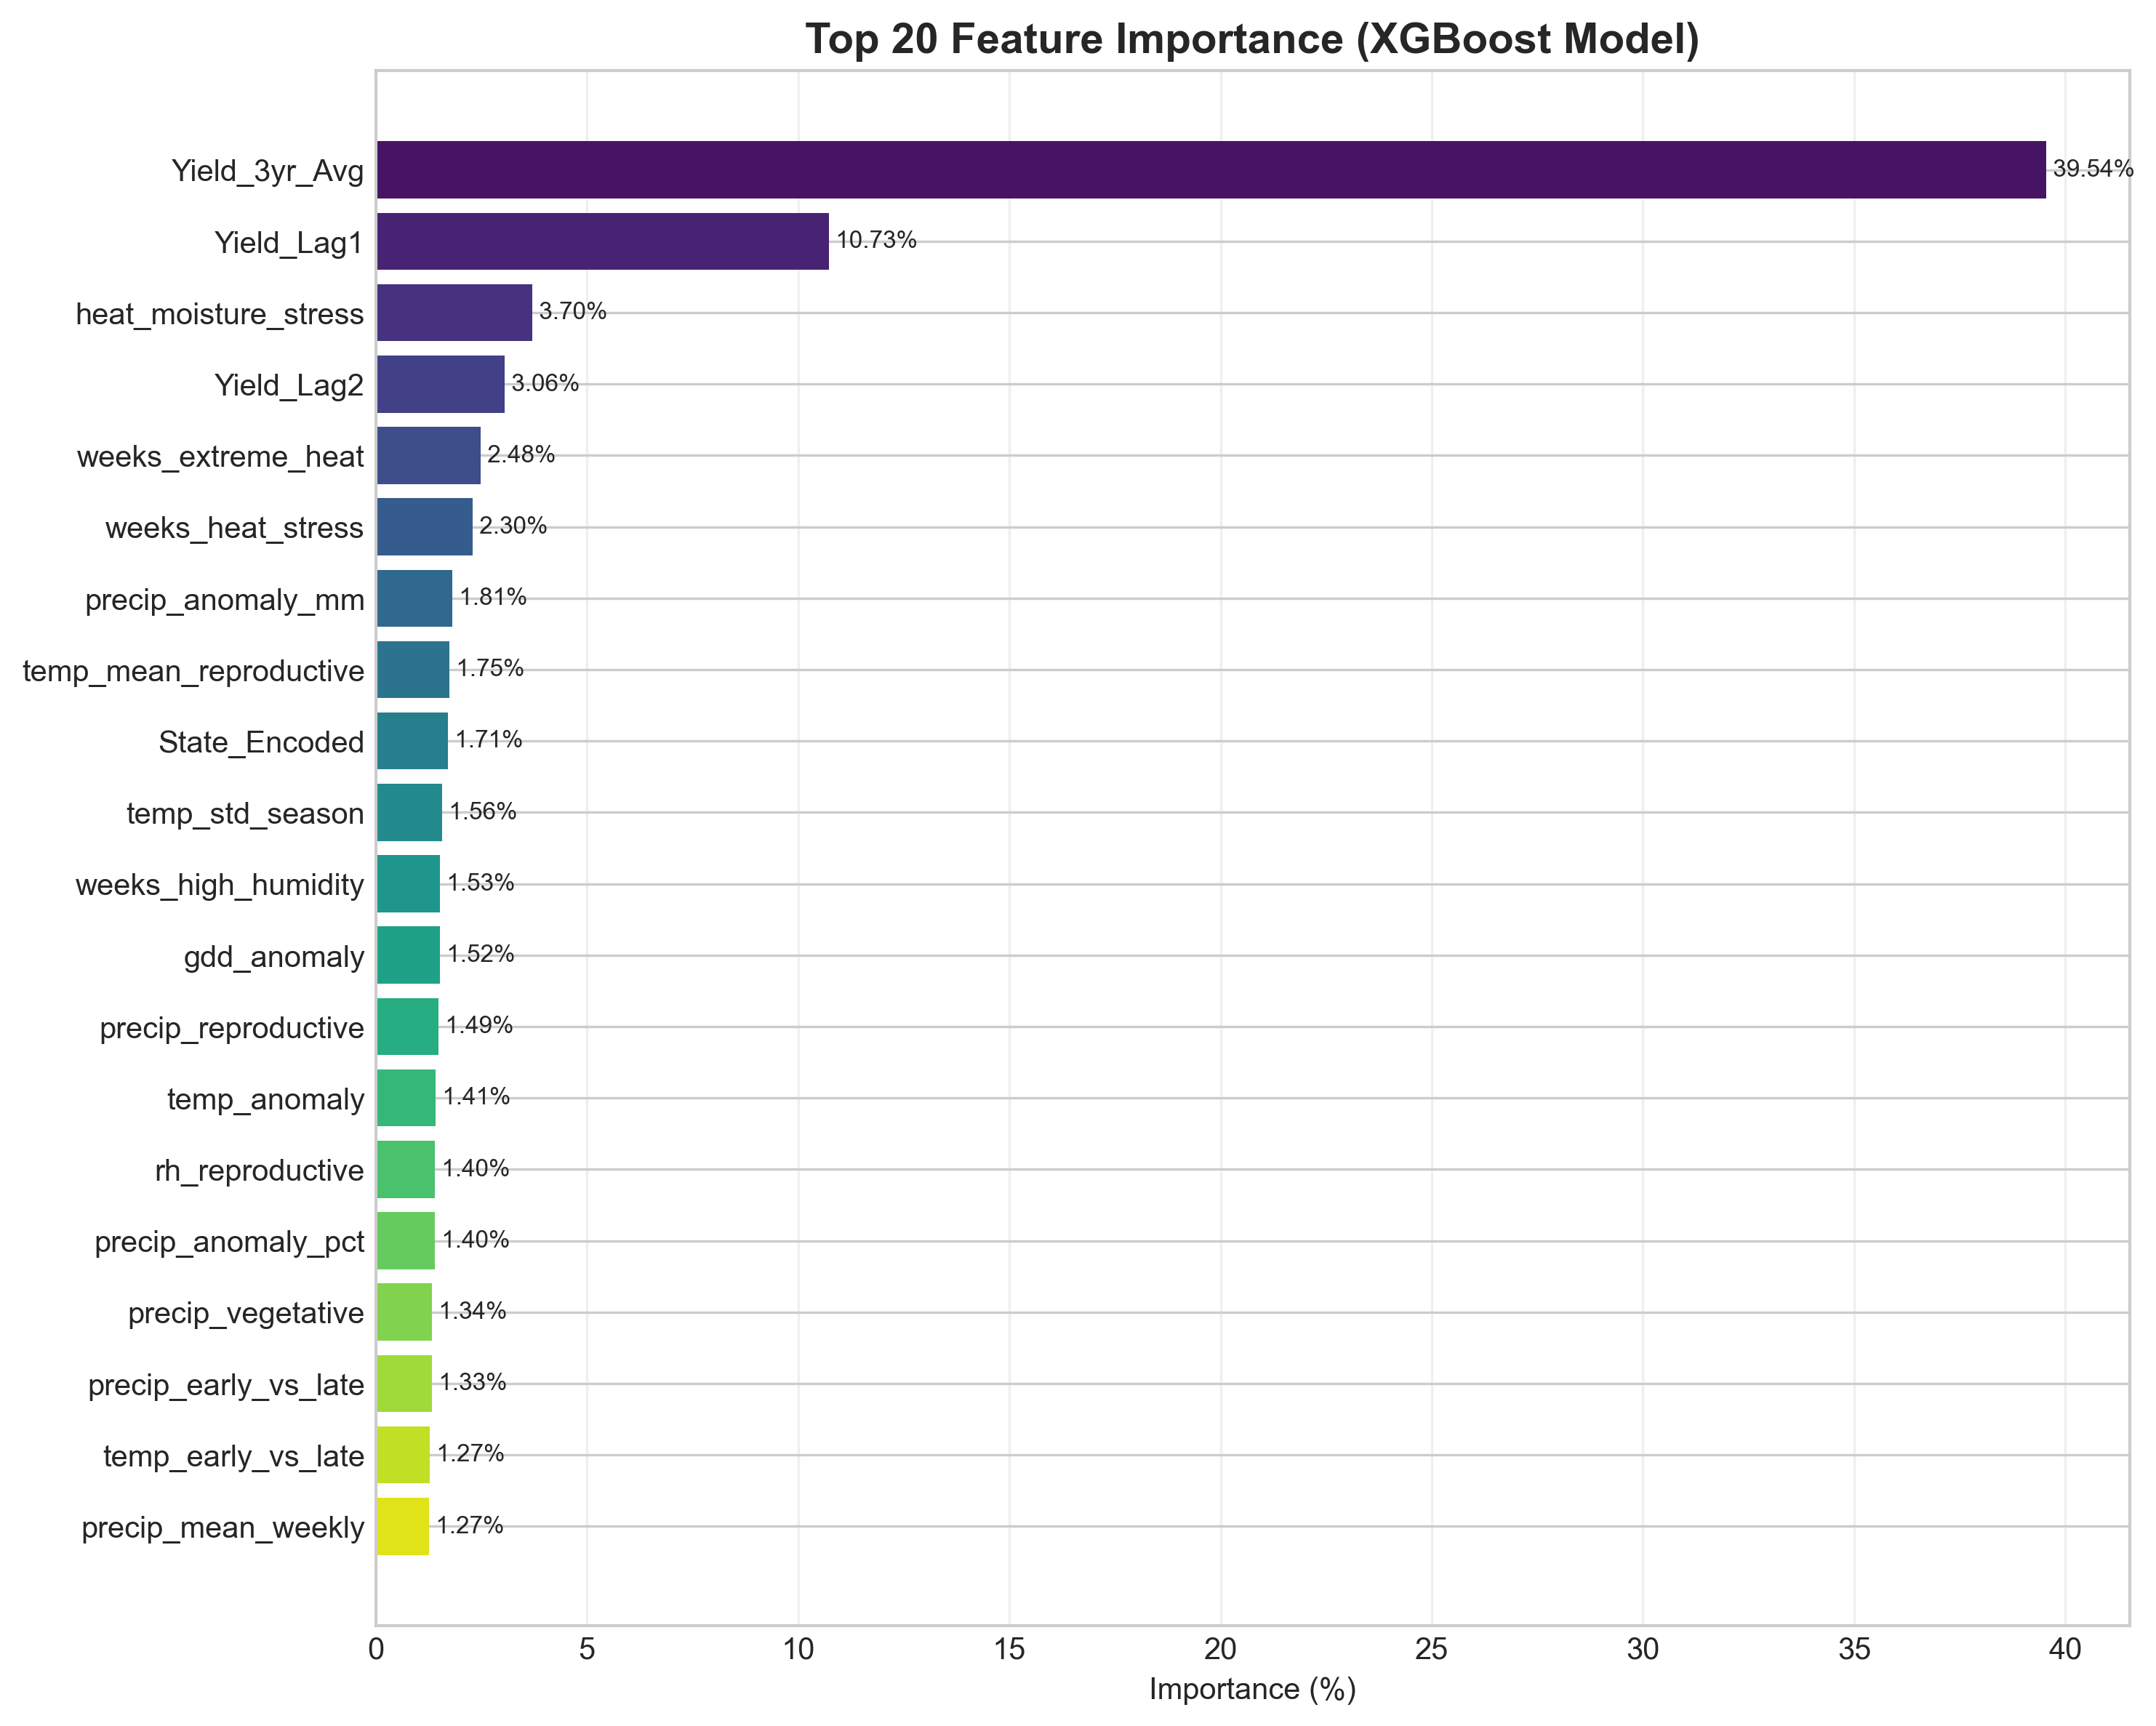
\includegraphics[width=\columnwidth]{figures/feature_importance.png}
\caption{Top 20 Feature Importance Scores from XGBoost Model}
\label{fig:feature_importance}
\end{figure}

\begin{figure}[htbp]
\centering
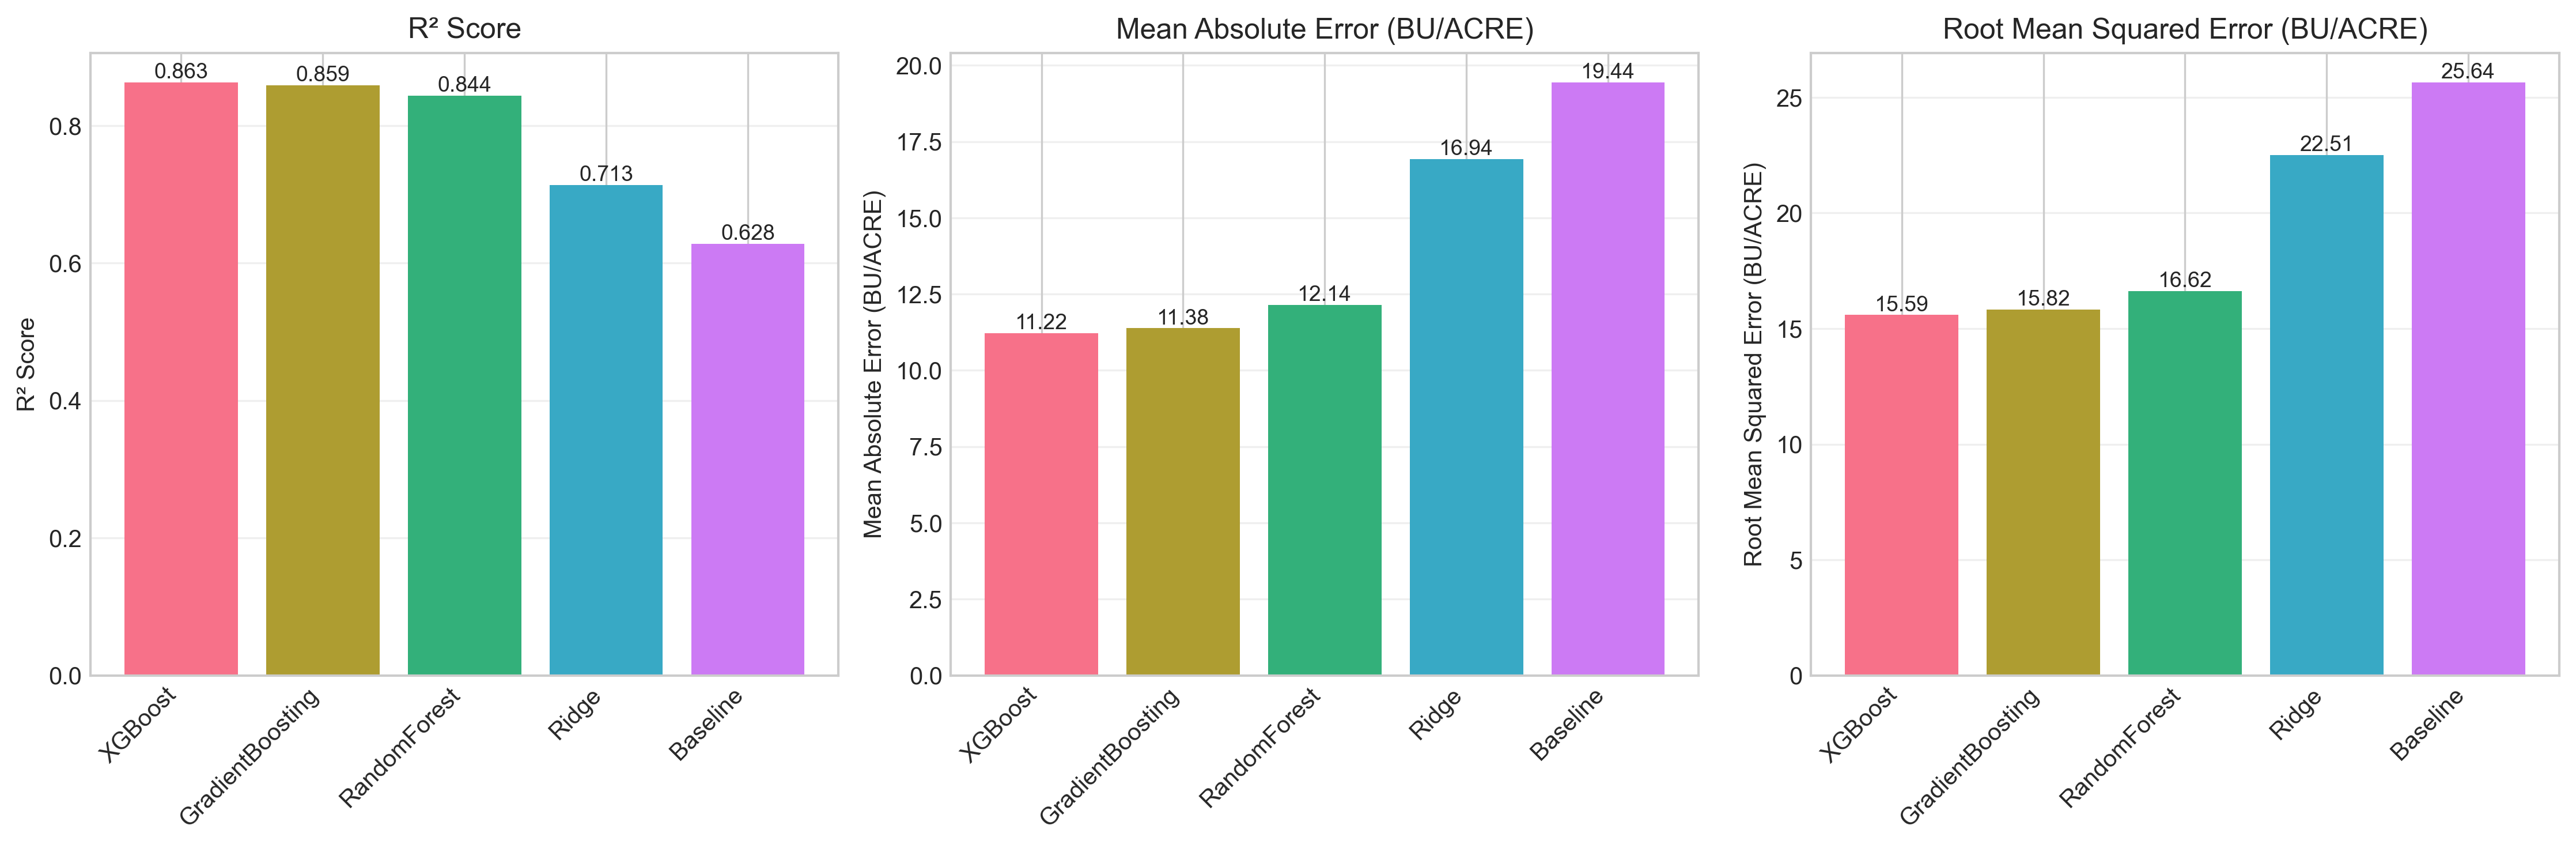
\includegraphics[width=\columnwidth]{figures/model_comparison.png}
\caption{Model Performance Comparison Across All Metrics}
\label{fig:model_comparison}
\end{figure}

\subsection{Error Analysis}

\subsubsection{Temporal Patterns}

Model performance varies across years, with best performance during 2020-2023 (MAE = 10.88 BU/ACRE) and worst performance during 2012 (MAE = 16.63 BU/ACRE), which experienced severe drought conditions across the corn belt. The model struggles during extreme weather events that fall outside the distribution of training data.

\subsubsection{Spatial Patterns}

Error analysis by state reveals geographic patterns in model performance. Table \ref{tab:error_by_state} shows MAE for selected states. Corn Belt states (Iowa, Illinois, Nebraska, Indiana) show lowest errors (MAE = 7-10 BU/ACRE), likely due to more stable growing conditions and better data availability. Peripheral states and regions with high yield variability show higher errors (MAE = 15-25 BU/ACRE). New Mexico shows the highest error (MAE = 25.0 BU/ACRE), likely due to limited corn production and high yield variability.

\begin{table}[htbp]
\caption{Mean Absolute Error by State (Top and Bottom 5 States by MAE)}
\label{tab:error_by_state}
\centering
\begin{tabular}{lcc}
\toprule
State & MAE (BU/ACRE) & Count \\
\midrule
\textbf{Lowest Errors:} & & \\
Indiana & 7.40 & 530 \\
Wisconsin & 8.45 & 392 \\
Iowa & 8.59 & 567 \\
Illinois & 8.62 & 598 \\
Minnesota & 9.03 & 485 \\
\midrule
\textbf{Highest Errors:} & & \\
New Mexico & 25.00 & 55 \\
Arizona & 19.91 & 21 \\
Montana & 18.77 & 61 \\
California & 18.00 & 92 \\
Oklahoma & 15.84 & 195 \\
\bottomrule
\end{tabular}
\end{table}

\subsubsection{Yield Level Patterns}

Table \ref{tab:error_by_yield} shows model performance across different yield levels. Interestingly, the model shows relatively consistent MAE across yield categories (10-13 BU/ACRE), but the relative error (MAPE) varies significantly. Very low yield counties (<100 BU/ACRE) show the highest relative error (MAPE = 18.7\%), while high yield counties (175-200 BU/ACRE) show the lowest relative error (MAPE = 6.1\%). This pattern suggests the model is optimized for typical production conditions, with increased uncertainty in marginal growing regions where yields are more variable.

\begin{table}[htbp]
\caption{Model Performance by Yield Level Categories}
\label{tab:error_by_yield}
\centering
\begin{tabular}{lccc}
\toprule
Yield Category & MAE (BU/ACRE) & MAPE (\%) & Count \\
\midrule
Very Low (<100) & 11.79 & 18.69 & 4,215 \\
Low (100-150) & 10.08 & 8.17 & 4,655 \\
Medium (150-175) & 11.79 & 7.30 & 1,596 \\
High (175-200) & 11.29 & 6.08 & 809 \\
Very High (>200) & 13.11 & 6.11 & 263 \\
\bottomrule
\end{tabular}
\end{table}

\begin{figure}[htbp]
\centering
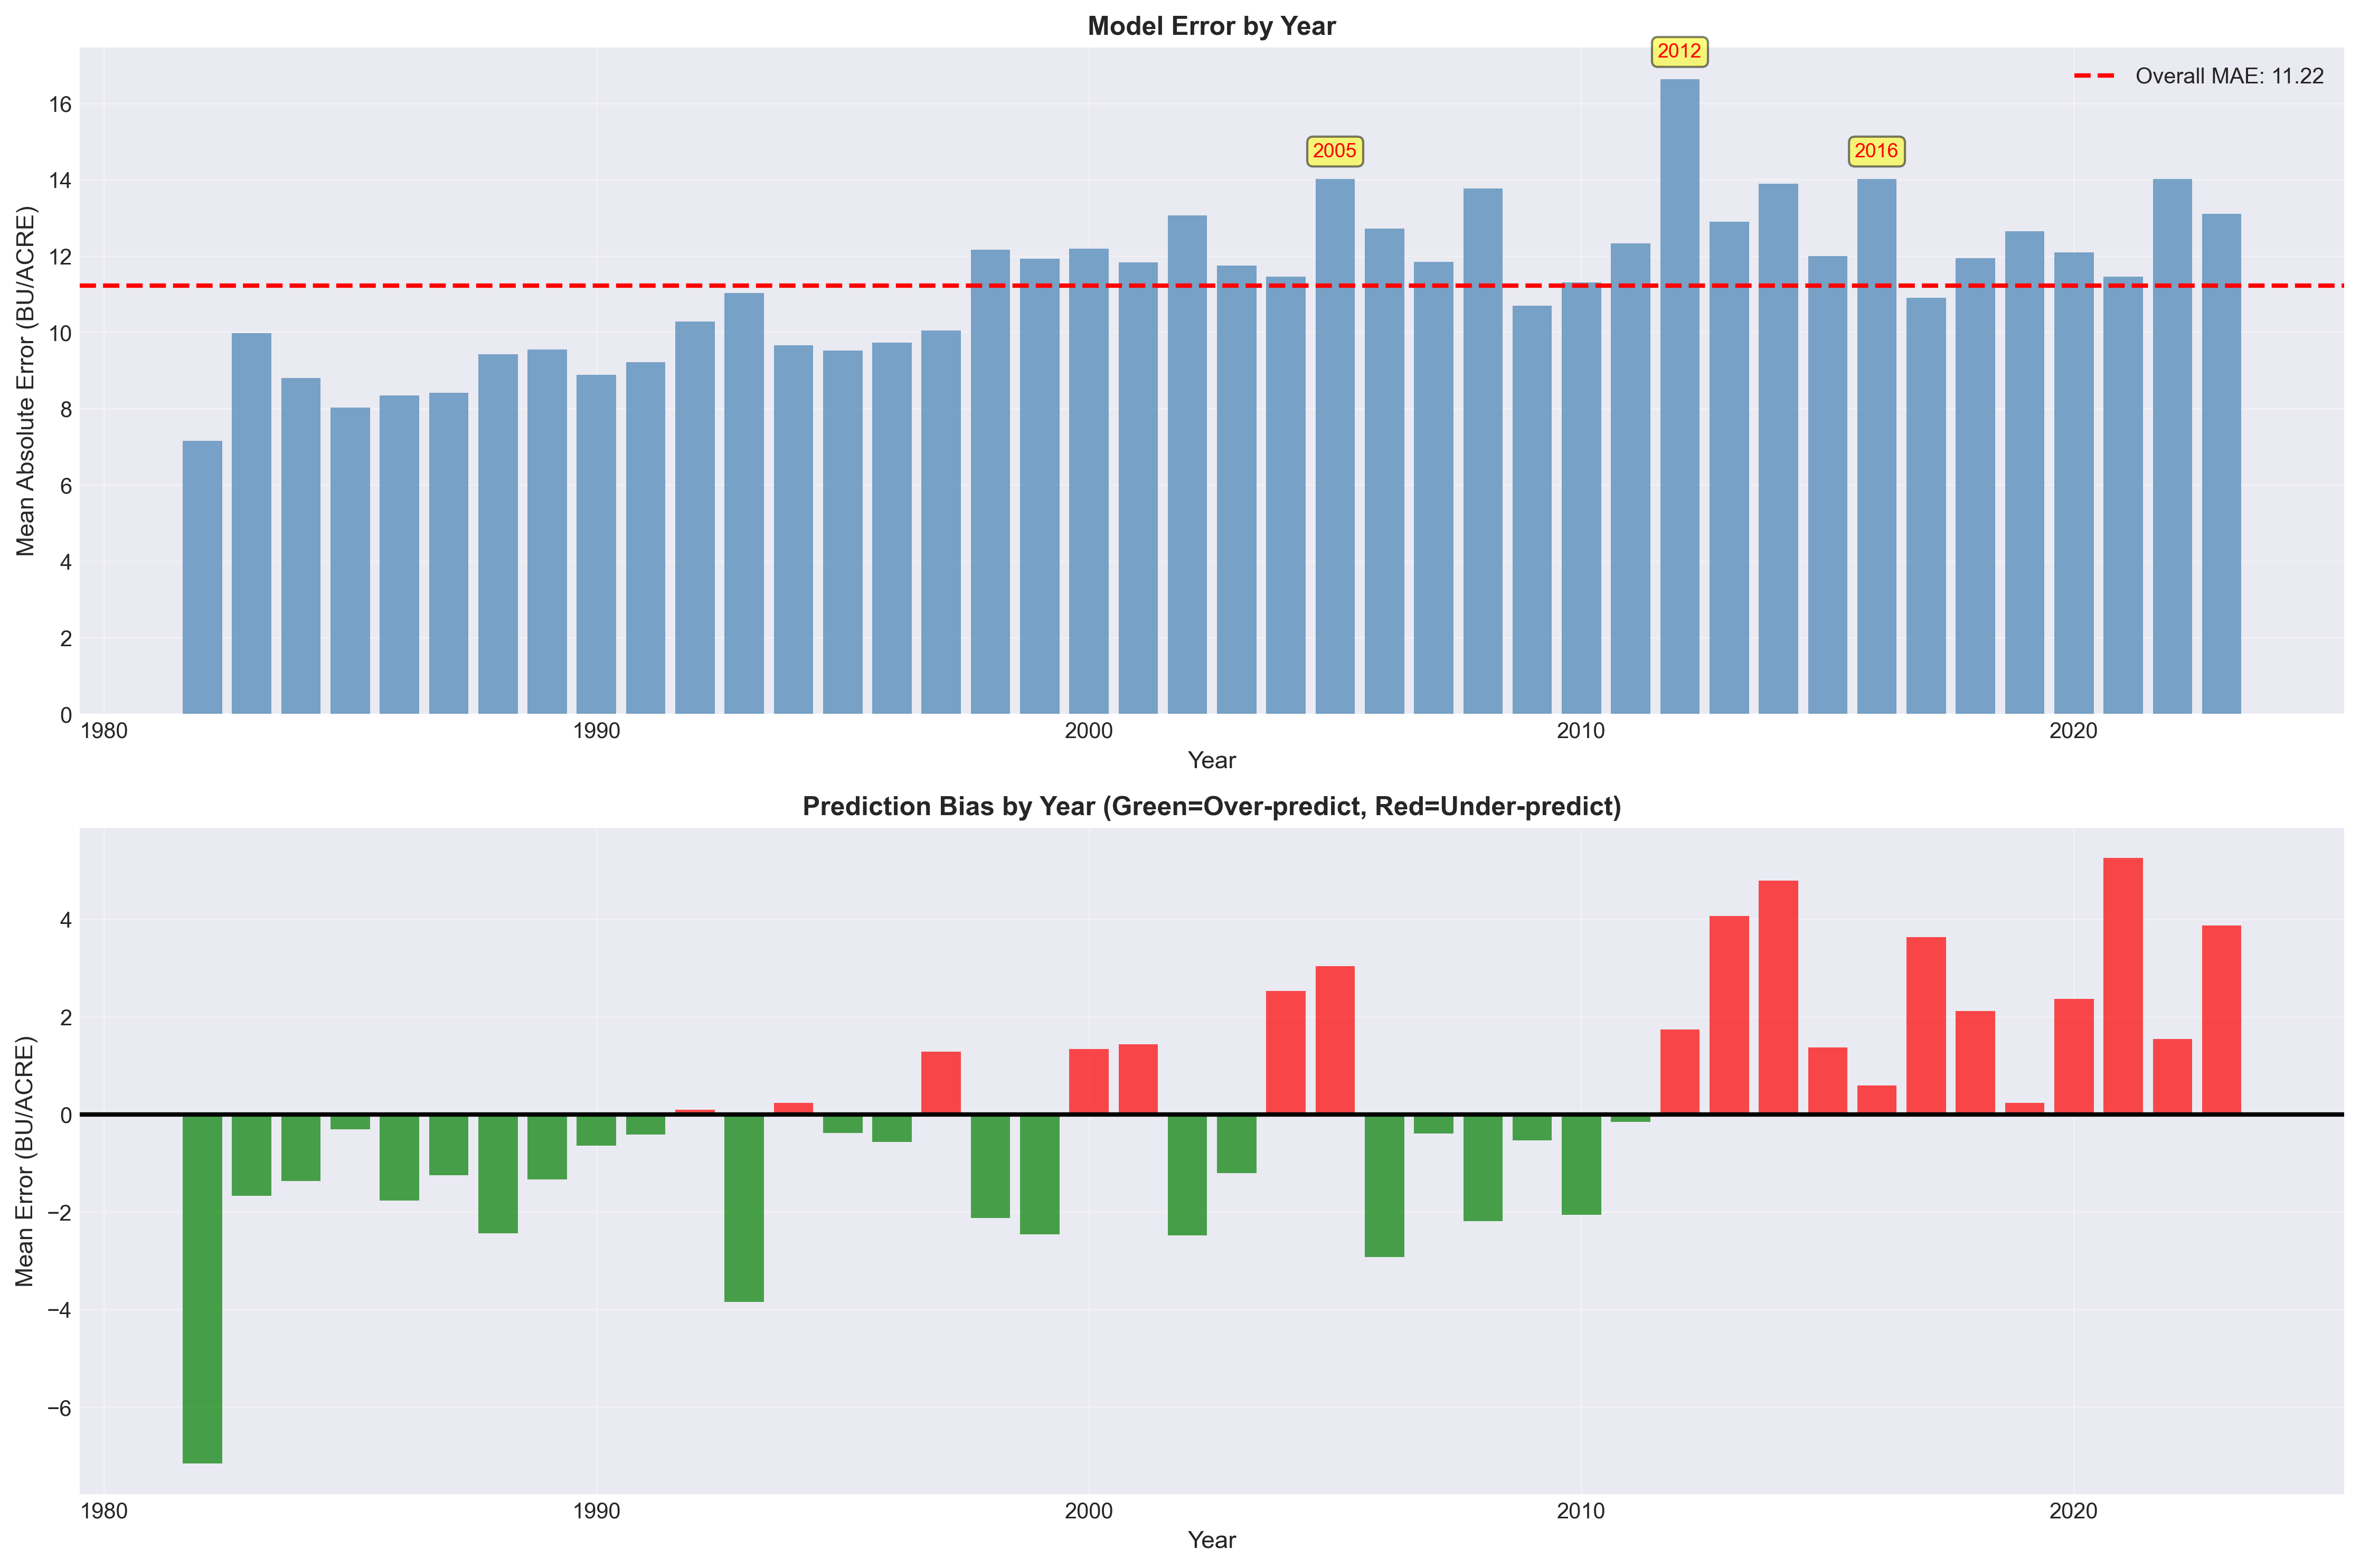
\includegraphics[width=\columnwidth]{figures/error_by_year.png}
\caption{Prediction Errors by Year (Test Set)}
\label{fig:error_by_year}
\end{figure}

\section{Proof of Concept}

We developed an interactive web application using Streamlit to demonstrate the practical utility of our yield prediction system. The application provides several key functionalities:

\textbf{Yield Prediction:} Users can select a county and year to obtain yield predictions with confidence intervals. The interface shows historical context and allows customization of weather and soil parameters.

\textbf{Scenario Analysis:} Users can explore "what-if" scenarios by adjusting weather conditions. Pre-defined scenarios include drought, optimal weather, extreme heat, and excessive rain. Results are compared to baseline predictions with visualizations.

\textbf{Data Exploration:} Interactive visualizations enable exploration of historical data with filtering by state, county, and year range. Geographic maps, trend charts, and distribution plots provide insights into yield patterns.

\textbf{Model Insights:} The application displays model comparison metrics, feature importance visualizations, and error analysis results, helping users understand model strengths and limitations.

The application is deployed and accessible at \url{https://us-corn-yield-ml.streamlit.app}, demonstrating the system's practical applicability for agricultural planning and decision-making. The complete source code and implementation are available at \url{https://github.com/AhsanRiaz786/us-corn-yield-ml}.

\section{Discussion}

Our results demonstrate the effectiveness of integrating multiple data sources and employing ensemble learning methods for corn yield prediction. The strong performance of historical yield features suggests that temporal persistence is a key factor, likely capturing long-term factors such as soil quality, management practices, and local adaptation.

The importance of climate anomalies over absolute values highlights the need to account for local conditions. Counties adapted to specific climates respond differently to the same absolute weather conditions, making anomaly-based features more predictive.

The superior performance of XGBoost can be attributed to its ability to capture complex non-linear relationships and feature interactions. The regularization mechanisms prevent overfitting while allowing the model to learn intricate patterns in the data.

Error analysis reveals important limitations. The model struggles during extreme events such as the 2012 drought, suggesting that training data may not adequately represent tail events. This is a common challenge in agricultural forecasting, where extreme weather events are rare but have significant impacts.

Spatial variation in errors suggests that regional differences in data quality, growing practices, or climate variability affect model performance. Future work could develop region-specific models or incorporate regional features to address these differences.

\section{Limitations and Future Work}

\subsection{Current Limitations}

Several limitations should be acknowledged:

\textbf{Temporal Resolution:} Our model predicts annual yields but does not provide in-season updates or sub-annual forecasts. Incorporating real-time data during the growing season could enable dynamic yield adjustments.

\textbf{Spatial Resolution:} County-level predictions may not capture sub-county heterogeneity in soils, management, or microclimates. Field-level predictions would require additional data sources.

\textbf{Data Limitations:} Weather data is extracted from county centroids rather than area-weighted averages, potentially missing spatial variability. Soil data is static and does not capture seasonal or management-induced changes.

\textbf{Extreme Events:} The model struggles during unprecedented weather events, as these fall outside the training distribution. Incorporating climate change projections or synthetic data augmentation could improve robustness.

\textbf{Management Practices:} We do not explicitly model management decisions such as planting dates, variety selection, or fertilizer application, which significantly influence yields.

\subsection{Future Work}

Several directions for future research are promising:

\textbf{Satellite Imagery:} Incorporating remote sensing data (NDVI, LAI, soil moisture) could provide real-time information about crop conditions and enable in-season yield adjustments.

\textbf{Deep Learning:} Long short-term memory (LSTM) networks could better capture temporal dependencies, while convolutional neural networks could process spatial patterns in satellite imagery.

\textbf{Economic Features:} Incorporating economic factors such as fertilizer prices, crop insurance, and market conditions could improve predictions by capturing management decision influences.

\textbf{Multi-Crop Extension:} Extending the framework to other major crops (soybeans, wheat) would demonstrate generalizability and enable comparative analysis.

\textbf{Uncertainty Quantification:} Developing probabilistic forecasts with confidence intervals would provide more actionable information for decision-making under uncertainty.

\textbf{Real-Time API:} Developing a production API with real-time data integration would enable practical deployment for agricultural applications.

\section{Conclusion}

This paper presents a comprehensive machine learning system for predicting county-level corn yields in the United States. By integrating data from USDA NASS, NASA POWER, and USDA NRCS, we create a rich feature set that captures historical patterns, weather conditions, and soil properties. Our evaluation demonstrates that ensemble methods, particularly XGBoost, achieve strong predictive performance with R² = 0.863 and MAE = 11.22 BU/ACRE.

Key findings include: (1) historical yield patterns are the strongest predictors, accounting for 53\% of feature importance; (2) climate anomalies are more predictive than absolute values, emphasizing the importance of local adaptation; (3) ensemble methods significantly outperform linear baselines by capturing non-linear relationships; and (4) model performance varies spatially and temporally, with higher errors during extreme events and in marginal growing regions.

The interactive web application demonstrates practical utility for agricultural planning and scenario analysis. While current limitations exist regarding extreme events and spatial resolution, the framework provides a solid foundation for future enhancements incorporating satellite data, deep learning, and economic factors.

Our work contributes to the growing body of research on data-driven agricultural forecasting and demonstrates the value of integrating heterogeneous data sources for improved prediction accuracy. The open-source implementation and comprehensive evaluation provide a foundation for future research and practical applications in precision agriculture.

\section*{Acknowledgment}

The authors acknowledge the data providers: USDA National Agricultural Statistics Service (NASS) for agricultural statistics, NASA POWER Project for weather data, USDA Natural Resources Conservation Service (NRCS) for soil data, and US Census Bureau for geographic data. This work was completed as part of CS 245 - Machine Learning course requirements.

The complete source code, trained models, and interactive dashboard are available in the project repository: \url{https://github.com/AhsanRiaz786/us-corn-yield-ml}. The interactive web application can be accessed at \url{https://us-corn-yield-ml.streamlit.app}.

\begin{thebibliography}{00}
\bibitem{schlenker2009nonlinear} W. Schlenker and M. J. Roberts, ``Nonlinear temperature effects indicate severe damages to U.S. crop yields under climate change,'' \textit{Proceedings of the National Academy of Sciences}, vol. 106, no. 37, pp. 15 594--15 598, 2009.

\bibitem{becker2019using} M. Becker-Reshef, C. Justice, M. Sullivan, E. Vermote, C. Tucker, A. Anyamba, and J. Small, ``Monitoring global croplands with coarse resolution earth observations: The global agriculture monitoring (GLAM) project,'' \textit{Remote Sensing}, vol. 2, no. 6, pp. 1589--1609, 2010.

\bibitem{crane2011forecasting} C. Crane-Droesch, ``Machine learning methods for crop yield prediction and climate change impact assessment in agriculture,'' \textit{Environmental Research Letters}, vol. 13, no. 11, p. 114003, 2018.

\bibitem{jeong2016random} J. H. Jeong, J. P. Resop, N. D. Mueller, D. H. Fleisher, K. Yun, E. E. Butler, D. J. Timlin, K. Shim, J. S. Gerber, V. S. Reddy, and S. H. Kim, ``Random forests for global and regional crop yield predictions,'' \textit{PLoS ONE}, vol. 11, no. 6, p. e0156571, 2016.

\bibitem{pantazi2016wheat} X. E. Pantazi, D. Moshou, T. Alexandridis, R. L. Whetton, and A. M. Mouazen, ``Wheat yield prediction using machine learning and advanced sensing techniques,'' \textit{Computers and Electronics in Agriculture}, vol. 121, pp. 57--65, 2016.

\bibitem{schwalbert2020forecasting} R. A. Schwalbert, T. Amado, G. Corassa, L. P. Pott, P. V. V. Prasad, and I. A. Ciampitti, ``Satellite-based soybean yield forecast: Integrating machine learning and weather data for improving crop yield prediction in southern Brazil,'' \textit{Agricultural and Forest Meteorology}, vol. 284, p. 107886, 2020.

\bibitem{wang2018deep} A. X. Wang, C. Tran, N. Desai, D. Lobell, and S. Ermon, ``Deep transfer learning for crop yield prediction with remote sensing data,'' in \textit{Proceedings of the 1st ACM SIGCAS Conference on Computing and Sustainable Societies}, 2018, pp. 1--5.

\bibitem{you2017deep} J. You, X. Li, M. Low, D. Lobell, and S. Ermon, ``Deep gaussian process for crop yield prediction based on remote sensing data,'' in \textit{Proceedings of the AAAI Conference on Artificial Intelligence}, vol. 31, no. 1, 2017.

\end{thebibliography}

\section*{Appendix}

\subsection*{A. Data Processing Pipeline}

The complete data processing pipeline includes the following steps:
\begin{enumerate}
    \item Download agricultural statistics from USDA NASS QuickStats API
    \item Download weather data from NASA POWER for county centroids
    \item Download soil data from USDA NRCS Soil Data Access
    \item Extract county centroids from US Census TIGER/Line data
    \item Spatial matching of weather data to counties
    \item Temporal alignment of all data sources
    \item Feature engineering and calculation
    \item Data quality checks and cleaning
    \item Temporal train/validation/test split
\end{enumerate}

\subsection*{B. Hyperparameter Ranges}

Detailed hyperparameter search spaces for each model:

\textbf{Ridge Regression:}
\begin{itemize}
    \item Alpha: \{0.1, 1.0, 10.0, 100.0, 1000.0\}
\end{itemize}

\textbf{Random Forest:}
\begin{itemize}
    \item n\_estimators: \{100, 200, 300, 400\}
    \item max\_depth: \{10, 20, None\}
    \item min\_samples\_split: \{2, 5, 10\}
    \item min\_samples\_leaf: \{1, 2, 4\}
    \item max\_features: \{'auto', 'sqrt', 'log2'\}
\end{itemize}

\textbf{Gradient Boosting:}
\begin{itemize}
    \item learning\_rate: \{0.01, 0.05, 0.1, 0.2, 0.3\}
    \item n\_estimators: \{100, 200, 300, 400, 500\}
    \item max\_depth: \{3, 5, 7, 10\}
    \item subsample: \{0.8, 0.9, 1.0\}
\end{itemize}

\textbf{XGBoost:}
\begin{itemize}
    \item learning\_rate: \{0.01, 0.05, 0.1, 0.2, 0.3\}
    \item max\_depth: \{3, 5, 7, 10\}
    \item min\_child\_weight: \{1, 3, 5, 7\}
    \item subsample: \{0.6, 0.8, 1.0\}
    \item colsample\_bytree: \{0.6, 0.8, 1.0\}
\end{itemize}

\end{document}